\centerline{
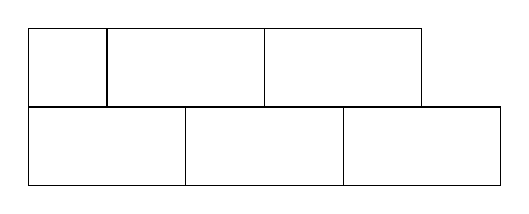
\begin{tikzpicture}
	\draw (0,0) --
		++(6,0) --
		++(0,1) --
		++(-6,0) --
		cycle;
	\draw (0,1) --
		++(0,1) --
		++(5,0) --
		++(0,-1);
	\draw (2,0) -- (2,1);
	\draw (4,0) -- (4,1);
	\draw (1,1) -- (1,2);
	\draw (3,1) -- (3,2);
\end{tikzpicture}}

A block wall $100$ feet long and $7$ feet high will be constructed using blocks that are $1$ foot high and either $2$ feet long or $1$ foot long (no blocks may be cut). The vertical joins in the blocks must be staggered as shown, and the wall must be even on the ends. What is the smallest number of blocks needed to build this wall?


\ifsat
	\begin{enumerate}[label=\Alph*)]
		\item 344
		\item 347
		\item 350
		\item 353%
	\end{enumerate}
\else
\fi

\ifacteven
	\begin{enumerate}[label=\textbf{\Alph*.},itemsep=\fill,align=left]
		\setcounter{enumii}{5}
		\item 344
		\item 347
		\item 350
		\addtocounter{enumii}{1}
		\item 353%
		\item 356
	\end{enumerate}
\else
\fi

\ifactodd
	\begin{enumerate}[label=\textbf{\Alph*.},itemsep=\fill,align=left]
		\item 344
		\item 347
		\item 350
		\item 353%
		\item 356
	\end{enumerate}
\else
\fi

\ifgridin
 353%

\else
\fi

